% =====================================================================
%  제출본 (submission) — 영문 단일 파일, 목표 12쪽
%
%  빌드:  pdflatex main.tex ; pdflatex main.tex
%
%  ■ 작업용 원고(../latex-en, ../latex)와 무엇이 다른가
%    내용을 줄인 판이다. 같은 정보를 본문·표·그림·캡션에서 여러 번 말하던 부분을
%    한 번만 말하도록 합쳤다:
%      · 그림 7 -> 3   (개념도·MLP·수요·짝비교 삭제, 아키텍처·분해·학습곡선만)
%      · 표   4 -> 2   (설정 통합표 · 주비교 통합표)
%      · 관련연구는 논문별 소개 -> 연구흐름 3문단
%      · 평가 프로토콜을 결과절에서 실험환경절로 옮김
%    수치는 작업용 원고와 같은 진단 대역(시드 9,900,950) 값이다.
%
%  ■ 국문판은 제출 폴더에 두지 않는다 (사용자 지시 2026-08-30).
%  ■ 머리말·쪽번호는 넣지 않는다 — 스프링거가 조판할 때 넣는다 (지침 §2.4·§4.1).
% =====================================================================
%  용지는 A4 로 둔다. 스프링거 지침이 용지 크기를 못 박지는 않지만 llncs 는
%  글 영역을 12.2 x 19.3 cm 로 고정하므로 A4 로 바꿔도 쪽수가 변하지 않고,
%  유럽 출판사·심사자 인쇄 환경에 맞는 쪽이 안전하다.
%  runningheads 는 넣지 않는다 — 지침 §2.4 "no need to include page numbers
%  or running heads; this will be done at our end."
\documentclass[a4paper]{llncs}

\usepackage[T1]{fontenc}
\usepackage[utf8]{inputenc}
\usepackage{graphicx}
\usepackage{booktabs}
\usepackage{amsmath, amssymb}
\usepackage{array}
\usepackage{caption}
\captionsetup{font=small}
\usepackage{marvosym}          % \Letter — 교신저자 표시
\usepackage{flafter}           % 부동체가 정의 지점보다 앞서 나오지 않게
\graphicspath{{figures/}}

\renewcommand{\topfraction}{0.9}
\renewcommand{\bottomfraction}{0.8}
\renewcommand{\textfraction}{0.07}
\renewcommand{\floatpagefraction}{0.75}
\setcounter{topnumber}{3}

\begin{document}
\raggedbottom

%  제목은 앞부분만 남긴다 (사용자 결정 2026-08-30) — 22단어는 LNCS 통상 범위(8~15)를
%  넘었다. 기여 둘(독립 제안·수락 정책 / 반사실 비용 학습)은 초록 첫 세 문장이 말한다.
%  "Smart" 는 뺐다: 평가가 합성환경이라 수식이 과하다 (keyword 에는 남겨 검색은 유지).
\title{A Reinforcement Learning Architecture for Spatio-Temporal
Reallocation in Real-Time Operations with Delayed Effects}
\titlerunning{RL Architecture for Spatio-Temporal Reallocation}

\author{Geon-U Kim \and Bong-Jun Choi\textsuperscript{\Letter}}
\authorrunning{G.-U. Kim and B.-J. Choi}
\institute{Department of Computer Engineering, Dongseo University,
Busan, Republic of Korea\\
\email{bongjun.choi@dongseo.ac.kr}}

\maketitle

% =====================================================================
\begin{abstract}
Container terminals assign each external-truck job to a yard block and
an appointment time before the truck arrives. A fixed assignment,
however, cannot account for congestion that emerges later. This paper
proposes a reinforcement learning architecture that jointly revisits the
block and the arrival time of an announced job during operation. Two
independent policies decide whether to propose a reallocation and
whether the destination block or time slot should accept it, and a
central procedure commits only mutually accepted candidates that satisfy
resource constraints. Moving one job affects not only that job but also
the waiting time of later trucks, the crane work sequence, and vessel
supply. To capture these delayed effects, each policy learns from cost
differences between discrete-event simulation branches that start from
the same state and differ in one action; online decisions use only the
trained networks. We evaluate the architecture in a continuous synthetic
environment whose time-of-day arrival variation follows the literature
and whose demand levels are design values. Compared with no
reallocation, the architecture reduced total operating cost by 14.7\%
over 28 days, and it achieved a lower cost than a rule-based policy with
the same spatio-temporal action range on 20 of 28 days ($p=0.036$).
Arrival-time adjustments accounted for 91.3\% of the reduction, and the
four most congested days for 90.5\%. These results suggest that
spatio-temporal reallocation may be more useful as a selective response
to observed congestion than as a continuous intervention.

\keywords{Smart port, Container terminal, Truck appointment system,
Yard block reallocation, Counterfactual cost learning, Reinforcement
learning}
\end{abstract}

% =====================================================================
\section{Introduction}
\label{sec:intro}
Container throughput continues to grow, but terminal land and equipment
cannot expand at the same rate, and the resulting pressure appears as
congestion in yard and gate operations. Studies of port efficiency show
that automation, intelligence, and environmental design affect
performance through different channels, so actual gains depend on how a
terminal translates observed information into operational
decisions~\cite{ref1}. Two research directions address this. On the
temporal side, truck appointment systems spread arrival peaks and let
terminals and carriers coordinate arrival times while retaining their
own costs~\cite{ref4,ref6}. On the spatial side, yard-operations
research improves container placement, work sequencing, and
crane-interference management~\cite{ref7,ref8,ref9,ref16}, and
reinforcement learning has been applied to real-time yard-crane
dispatching~\cite{ref19}.
Most of these approaches assume that the assigned yard block and
appointment time are fixed before the truck arrives and improve
operations within that assignment. During operation, however, demand may
concentrate in particular time slots or blocks while crane queues
change, so an assignment that was reasonable when announced may become
inefficient. This paper revisits the assignment itself: for an announced
job it jointly decides \emph{where} the job should be handled and
\emph{when} the truck should arrive. Moving one job affects later truck
queues, the crane work sequence, and vessel supply, so the immediate
cost of reallocation cannot capture its effect; difference rewards and
multi-agent counterfactual baselines address exactly this by comparing
one action with an alternative~\cite{ref10,ref11}. The destination must
also decide whether it can absorb the job, separately from any benefit
to the proposing side, so we use independent proposal and acceptance
policies while a central procedure checks mutual consent and
feasibility. Fig.~\ref{fig:arch} summarises the online decision path and
the offline counterfactual learning procedure.
This study makes three contributions: (i) a post-assignment
spatio-temporal reallocation architecture with independent proposal and
acceptance policies and a central commitment step; (ii) simulator-based
counterfactual cost learning that keeps expensive branch simulation
offline and leaves only small networks and constraint checks online; and
(iii) an evaluation that separates the effect of the action range from
the effect of learning, and that reports both how often and by how much
the learned policy is cheaper. The architecture is stated for real-time operational systems in which
an assignment can be revised while its consequences appear only later,
and it is instantiated and evaluated here in a container-terminal
environment.
Sect.~\ref{sec:related} reviews related
work, Sect.~\ref{sec:arch} presents the architecture and the learning
signal, Sect.~\ref{sec:env} describes the environment and the evaluation
protocol, and Sect.~\ref{sec:exp} reports the results.

% =====================================================================
\section{Related Work}
\label{sec:related}
Truck-appointment studies reshape demand in time: appointment windows
relieve gate congestion by redistributing arrivals rather than adding
capacity~\cite{ref4}, distributed formulations let carriers and the
terminal coordinate schedules while each keeps its own
cost~\cite{ref6}, and time-of-day models built from terminal records
show that arrivals are far from uniform over a day~\cite{ref13}.
Yard-operations studies reshape demand in space: crane work sequencing
reduces truck waiting~\cite{ref7}, multi-crane interference extends the
scheduling problem~\cite{ref8}, block length and crane deployment govern
terminal-wide performance under long simulations~\cite{ref9}, and the
relative standing of dispatching rules depends on terminal
conditions~\cite{ref16}. Both streams optimise operations after
the block and the appointment have been assigned; efficiency studies
suggest that the decision layer that produces those assignments is
itself a lever~\cite{ref1}.
Reinforcement learning has entered this domain at the execution layer:
a method based on proximal policy optimisation schedules yard cranes
in real time across multiple blocks~\cite{ref19}. We address the preceding
assignment layer, where the block and the arrival time are selected.
When several actors decide jointly, the future cost is a joint outcome
and the contribution of one action is hard to isolate. Difference
rewards construct a payoff that is aligned with the global objective yet
sensitive to the individual action~\cite{ref10}, and counterfactual
multi-agent baselines compare one actor's action with an alternative
while holding the rest fixed~\cite{ref11}. We follow this idea, but the
baseline is produced by re-simulating the terminal rather than by a
learned critic.
Two modelling choices follow. First, the networks do not output action
probabilities; each maps a state and one candidate action to a cost
score, and the policy selects the lowest score. The score is not an
absolute cost: labels are centred within each counterfactual pair
(Sect.~\ref{sec:arch-labels}), so a network learns what one action costs
relative to the action it was compared against. The method
therefore learns a value-like quantity rather than a policy; unlike deep
Q-networks, which bootstrap from their own estimates~\cite{refmnih}, the
target here is a Monte-Carlo cost difference measured over a fixed
horizon. Second, the approximator is a small multilayer perceptron.
Feedforward networks are general approximators~\cite{refhornik}, and the
input structure supports the choice. The delayed effect enters through
the label, which is a forward simulation over a fixed horizon, rather
than through the policy input: each candidate is scored from a
fixed-length vector of the current state, candidates are scored
independently, and the number of labels is small.

% =====================================================================
\section{Proposed Architecture}
\label{sec:arch}

\begin{figure}[bp]
\centering
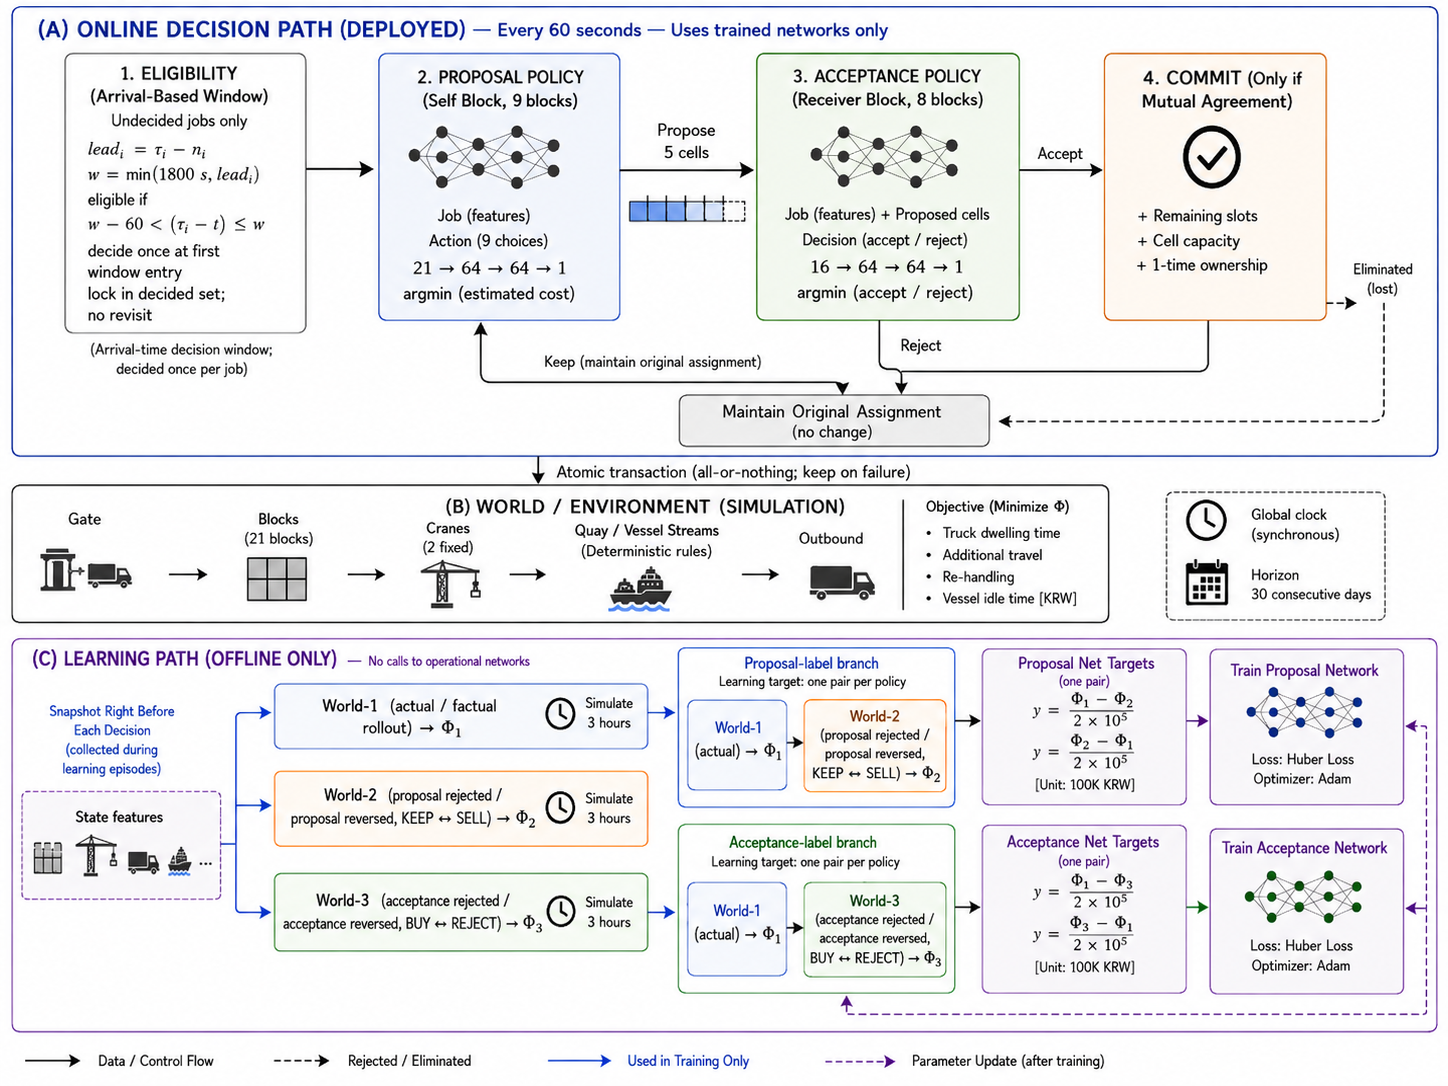
\includegraphics[width=\textwidth]{system-architecture.png}
\caption{The proposed architecture. (a) Every 60\,s the operational path
checks eligibility, proposal, acceptance, and commitment; failure of
mutual consent or capacity keeps the original assignment. (b) The
discrete-event environment links the gate, 21 blocks, two yard cranes
per block, and vessel operations to calculate the cost $\Phi$.
(c) Offline learning compares up to three worlds from the same state and
random stream over 3\,h and builds separate labels for the proposal and
acceptance cost networks.}
\label{fig:arch}
\end{figure}

\subsection{Notation, Actions, and Policies}
\label{sec:arch-notation}
The decision interval is $\delta=60$\,s. The current assignment of job
$i$ is $z_i=(b_i,\tau_i)$, where $b_i$ is the block and $\tau_i$ the
announced arrival time. A reallocation action
$a_i=(b'_i,\Delta_i)\in\mathcal A_i(t)$ gives
$z_i(a_i)=(b'_i,\tau_i+\Delta_i)$; keeping the assignment is
$a_i^0=(b_i,0)$. Block reallocation has $b'_i\ne b_i$ and arrival-time
adjustment has $\Delta_i>0$, and a candidate may change both. Outbound
jobs are excluded from block reallocation because the retrieved
container has a fixed location. Let $n_i$ be the announcement time,
$g_i$ the gate-in time, and $r_i$ an indicator of prior review. A job
becomes eligible not when it is announced but when its arrival comes
within a review window $w_i=\min(W,\ \tau_i-n_i)$ of the present, with
$W=1800$\,s. This delays the decision until the latest feasible point
before arrival, so the policy uses a more recent observation of terminal
conditions:

\begin{equation}
\mathcal E_t=\{i\mid w_i-\delta<\tau_i-t\le w_i,\ g_i>t,\ r_i=0\}.
\end{equation}
Each job therefore enters exactly one decision interval and is never
revisited. For a job announced at least $W$ ahead of its arrival the
decision falls exactly $W$ before that arrival, about 46 minutes later
than the median announcement; a job announced with a shorter lead is
reviewed immediately. A job announced no earlier than its own arrival
has $w_i=0$ and is never eligible; such jobs are 14.1\% of the demand,
and the architecture leaves them untouched. The proposal policy scores
each candidate from the block state and job-action features $o_i^P$ and
selects the lowest score, while the acceptance policy compares
acceptance with rejection from the proposal message and the destination
state $o_i^A$:

\begin{equation}
\begin{aligned}
\hat a_i&=\arg\min_{a\in\mathcal A_i(t)}
\hat c_{\theta}^{P}(o_i^P,a),\qquad
p_i=\mathbf 1[\hat a_i\ne a_i^0],\\
q_i&=\mathbf 1\!\left[
\hat c_{\psi}^{A}(o_i^A,\hat a_i,\mathrm{acc})
\le
\hat c_{\psi}^{A}(o_i^A,\hat a_i,\mathrm{rej})
\right].
\end{aligned}
\end{equation}
If the target resource has no remaining capacity, the request is
rejected before the network is called. The mutually accepted candidates
form $\mathcal J_t=\{i\in\mathcal E_t\mid p_iq_i=1\}$.

\subsection{Central Commitment}
\label{sec:arch-commit}
The central procedure creates no new candidates. It considers only
$\mathcal J_t$, sorted by the acceptance policy's predicted cost with
lexicographic tie-breaking. With $x_i\in\{0,1\}$ indicating commitment,
$F_b(t)$ the free slots in block $b$, and $K_k(t)$ the remaining quota
of time slot $k$, it enforces

\begin{equation}
\begin{aligned}
x_i&\le p_iq_i,\qquad
\sum_{i\in\mathcal J_t}\!x_i\mathbf1[b'_i\!=\!b]\le F_b(t),\\
\sum_{i\in\mathcal J_t}\!x_i\mathbf1[k(i)\!=\!k]&\le K_k(t),\qquad
\sum_{t\in\mathcal T}\!\mathbf1[i\in\mathcal E_t]\le1.
\end{aligned}
\end{equation}
Block capacity is enforced in every experiment; when time-slot quota
data are unavailable we set $K_k(t)=\infty$, so the arrival-time results
represent the potential range of adjustment rather than an executable
schedule. All committed assignments are applied together at the end of
the decision epoch, so an earlier commitment cannot change the state
seen by another candidate in the same epoch.

\subsection{Cost Networks}
\label{sec:arch-models}
Both $\hat c^{P}_{\theta}$ and $\hat c^{A}_{\psi}$ are multilayer
perceptrons with two 64-unit hidden layers and ReLU, with weights shared
across blocks: $21\to64\to64\to1$ for proposal and $16\to64\to64\to1$
for acceptance, or fewer than 11{,}000 parameters in total. Inputs
include current waiting, inventory, remaining crane work, the public
expected arrival time, route difference, and announced volume near the
target time; unrealised arrival and completion times and simultaneous
responses from other accepting parties are excluded. The output is one
pair-centred cost score per candidate, so the length of the candidate
list may change without retraining. Mean subtraction inside a pair
removes a constant that is common to both actions and therefore leaves
the ranking in~(2) unchanged.

\subsection{Counterfactual Cost Labels and Training}
\label{sec:arch-labels}
For each sampled decision we clone the state and the random stream just
before branching and run up to three worlds for $H=10{,}800$\,s:
$\phi_i^F=\Phi_H(\text{observed})$,
$\phi_i^P=\Phi_H(\text{proposal reversed})$, and
$\phi_i^A=\Phi_H(\text{acceptance reversed})$. The counterfactual branch
reverses the policy's observed decision: if the proposal policy proposed
a change the alternative keeps the assignment, if it kept the assignment
the alternative commits the cheapest candidate under the current
weights, and the acceptance alternative swaps acceptance and rejection.
For each policy the two actions of the pair are centred on their mean
and divided by KRW 100{,}000,

\begin{equation}
\bar\phi_i^P=\frac{\phi_i^F+\phi_i^P}{2},\quad
y_{i,F}^P=\frac{\phi_i^F-\bar\phi_i^P}{10^5},\quad
y_{i,P}^P=\frac{\phi_i^P-\bar\phi_i^P}{10^5},
\end{equation}
that is, $\pm$ half the pairwise cost difference; the same centring is
applied to $(\phi_i^F,\phi_i^A)$. The reference point is therefore the
pair itself rather than a fixed action.
We sample at most 64 decisions per day, split them 80/20 into training
and validation, and optimise with Adam ($3\times10^{-4}$) and Huber loss
($\beta=1.0$), which prevents a few very large counterfactual
differences from dominating the fit~\cite{refhuber}. Exploration
decreases linearly from 0.50 to 0.05 over the 30 training iterations.
The labels are not a fixed dataset: every pair branches from the action
the current policy actually took, so both the labelled states and the
alternative they are compared against move as the weights change, and
each iteration's labels are discarded after its update. In this respect
the scheme is on-policy Monte-Carlo advantage estimation with a
simulator-generated baseline; it uses neither bootstrapping nor a policy
gradient. Training both networks for 30 iterations took about 18 hours
of wall-clock time. During evaluation the weights are frozen,
exploration is disabled, and no counterfactual branch is called, so
online operation costs one forward pass per candidate.

% =====================================================================
\section{Experimental Environment and Evaluation Protocol}
\label{sec:env}
We evaluate the architecture in a literature-based synthetic environment
rather than in the operating record of a particular terminal. The
studies of Sect.~\ref{sec:related} provide the modelling ranges---a
yard of roughly twenty blocks~\cite{ref16}, multiple cranes per block~\cite{ref8}, continuous
multi-week operation~\cite{ref9}, strong time-of-day variation in truck
arrivals~\cite{ref13}, three vessel classes~\cite{ref16}, and a reported
range of crane handling times~\cite{ref9}---and Table~\ref{tab:setup}
lists the values used within them. Following the practice of separating
measured ranges from synthetic parameters and identifying the synthetic
component explicitly~\cite{ref20}, we state which values are design
choices: the daily demand levels, the shape of the arrival curve, the
counterfactual horizon, and two of the four cost coefficients.

\begin{table}[tbp]
\centering
\caption{Experimental setup. Values marked \emph{design} are choices of
this study; the others lie within ranges reported in the cited work.
Job announcement times follow
$f(t)=0.38\,U(0,24)+0.62\sum_{m=1}^{3}w_m\mathcal N(t;\mu_m,\sigma_m^2)$
with $(\mu_m,\sigma_m,w_m)$ equal to $(10,1.5,.317)$, $(15,2.5,.633)$,
and $(21,1,.05)$, time in hours.}
\label{tab:setup}
\small
\setlength{\tabcolsep}{4pt}
\begin{tabular}{@{}l l@{\hspace{0.9em}} l@{}}
\toprule
Group & Setting & Value \\
\midrule
Yard & Blocks, cranes per block & 21, 2 \\
 & Slots per block, initial occupancy & 1{,}440, 65\% \\
\midrule
Time & Decision interval $\delta$ & 60\,s \\
 & Review window $W$ & 1{,}800\,s \\
 & Counterfactual horizon $H$ (design) & 10{,}800\,s \\
\midrule
Demand & Announcement lead & median 1.27\,h (14.1\% $\le0$) \\
 & Daily levels (design) & 3{,}500, 5{,}000, 7{,}500, 12{,}500, 15{,}000 \\
 & Draw probabilities (design) & 0.30, 0.30, 0.25, 0.10, 0.05 \\
 & Arrival curve (design) & uniform base 38\% $+$ 3 Gaussians \\
\midrule
Vessels & Classes (GT), calls/day, crane rate & 50/100/150k, 3.3, 27.5 moves/h \\
\midrule
Cost & Truck dwell & KRW 40{,}000/h (twice beyond 1\,h) \\
 & Crane move, rehandle (design) & KRW 60{,}000/h, KRW 2{,}000/event \\
 & Vessel idling & KRW 2.99 per GT-hour~\cite{ref25} \\
\midrule
Learning & Networks (proposal, acceptance) & $21/16\!\to\!64\!\to\!64\!\to\!1$ \\
 & Iterations, decisions per day & 30, $\le64$ \\
 & $\varepsilon$, optimiser & $0.50\!\to\!0.05$, Adam $3\times10^{-4}$ \\
\midrule
Evaluation & Days, compared, seed & 30, middle 28, 9{,}900{,}950 \\
 & Policy at evaluation & frozen weights, $\varepsilon=0$ \\
\bottomrule
\end{tabular}
\end{table}

The total cost over $[d,d+1)$ is the sum of four terms, where $h_i$ is
the dwell time of truck $i$, $m$ the additional crane working time, $R$
the number of rehandles, and $T_v$ the policy-related idle time of
vessel $v$:

\begin{equation}
\begin{aligned}
\Phi_d&=C_{wait,d}+C_{move,d}+C_{rehandle,d}+C_{vessel,d},\\
C_{wait}&=\sum_i 40{,}000\{h_i+\max(0,h_i-1)\},\qquad
C_{move}=60{,}000\,million,\\
C_{rehandle}&=2{,}000\,R,\qquad
C_{vessel}=\sum_v 2.99\,GT_v T_v.
\end{aligned}
\end{equation}
The base monetary scale is
derived from the safe trucking freight rate~\cite{ref24}, whereas the
conversion to an hourly dwell-cost coefficient is a design choice.
Structural vessel time that the policy cannot change is recorded
separately. Waiting dominates the total: $C_{wait}$ accounts for 96.4\%,
against 2.2\% for rehandling, 1.2\% for vessel idling, and 0.1\% for
crane movement, so conclusions based on $\Phi$ are driven mainly by the
truck dwell coefficient. Congestion changes the cost structure as well
as its level: waiting is 83.2\% of cost at 3{,}500 trucks per day and
99.1\% at 15{,}000, and the daily 90th-percentile turn time ranges from
0.79\,h on the lightest days to 7.49\,h on the heaviest.
The evaluation uses a 30-day continuous run with a random seed held
out from training; the middle 28 days are
compared and the first and last days only connect the continuous
boundaries. All policies share the same truck, vessel, and service
random streams on a given day, following the common-random-number
method~\cite{ref22}. Implementation checks confirm that proposal and acceptance use separate
models, that one-sided consent never produces a commitment, that realised
future times
are excluded from policy inputs, and that state continues across day
boundaries; frozen-policy evaluation made zero counterfactual calls, and
a branch that changed no action reproduced the main run at all four
sampled points. We compare the learned policy with three groups:
its own ablations, which allow only arrival-time adjustment or only
block reallocation; the model after the first of the 30 training
iterations, which isolates the effect of the remaining iterations; and
six rule-based policies, four of which reallocate blocks
(least slack, first-come-first-served, shortest processing time, net
gain) while two transfer the \emph{least-loaded} criterion to the
temporal axis and therefore match the spatio-temporal action range of
the learned policy.

% =====================================================================
\section{Results}
\label{sec:exp}

\subsection{Cost Reduction and Paired Daily Comparison}
\label{sec:exp-paired}
Over the 28 compared days, total cost was KRW 10.00\,billion without
reallocation and KRW 8.52\,billion with the learned policy, a reduction of
KRW 1.471\,billion or 14.7\% (Table~\ref{tab:main}). Days are treated as
independent comparison units, and we report two paired tests because
they answer different questions. A two-sided sign test counts only the
days on which one policy is cheaper, so it is blind to how large each
day's difference is; a Wilcoxon signed-rank test ranks the differences
by magnitude before summing them, so a policy that wins on fewer days
but by a wider margin is scored differently by the two tests. The
distinction
matters here because the learned policy acts selectively. With 28 days
and no tied differences, both tests are computed exactly.

\begin{table}[tbp]
\centering
\caption{Main comparison. ``Reduction'' is the 28-day total against no
reallocation; positive means lower cost. The paired columns compare the
learned policy with that row's policy on the same days, and $p$ values
are two-sided and exact. Values below 0.05 are in bold. Against no
reallocation the two days on which the learned policy is more expensive
cost KRW $-17.1$\,million and KRW $-0.5$\,million, whereas each of the four
congested days exceeds KRW 290\,million.}
\label{tab:main}
\footnotesize
\setlength{\tabcolsep}{4pt}
\begin{tabular}{@{}l@{\hspace{0.7em}} l@{\hspace{0.7em}} r@{\hspace{1em}} c@{\hspace{0.7em}} r@{\hspace{0.6em}} r@{}}
\toprule
Policy & Actions & Reduction &
\shortstack{Learned\\cheaper} & \shortstack{Sign\\$p$} &
\shortstack{Rank\\$p$} \\
\midrule
\textbf{Learned policy} & block+time & \textbf{+14.72\%} & --- & --- & --- \\
Learned, time only & time & +13.44\% & --- & --- & --- \\
Learned, block only & block & $-$1.31\% & --- & --- & --- \\
\midrule
First-iteration model & block+time & +7.97\% & 18/28 & 0.185 & 0.164 \\
\midrule
Rule: least-loaded slot & time & +3.41\% & --- & --- & --- \\
Rule: least-loaded block+slot & block+time & +1.51\% & 20/28 & \textbf{0.036} & \textbf{0.015} \\
Rule: least slack & block & +0.53\% & 20/28 & \textbf{0.036} & \textbf{$<$0.001} \\
Rule: first-come-first-serve & block & +0.17\% & 22/28 & \textbf{0.004} & \textbf{$<$0.001} \\
Rule: shortest processing time & block & +0.05\% & 21/28 & \textbf{0.013} & \textbf{0.006} \\
Rule: net gain & block & $-$0.48\% & 21/28 & \textbf{0.013} & \textbf{0.003} \\
\midrule
No reallocation & --- & 0.00\% & 26/28 & \textbf{$<$0.001} & \textbf{$<$0.001} \\
\bottomrule
\end{tabular}
\end{table}

The learned policy costs less than the rule with the same
block-and-time action range on 20 of 28 days (sign test $p=0.036$,
signed-rank $p=0.015$), and less than no reallocation on 26 of 28 days
($p<0.001$). It costs less than the first-iteration model on 18 days,
but this difference is not statistically significant under either test
($p=0.185$ and $p=0.164$). At the 5\% level the two tests agree on every
row of Table~\ref{tab:main}, although the signed-rank $p$ is the smaller
of the two in most rows, which is consistent with an effect concentrated
in a small number of high-cost days.
The temporal comparison shows why both tests are needed.
Restricted to arrival-time adjustment, the rule that transfers the
least-loaded criterion to the temporal axis reduces cost by 3.41\%
relative to no reallocation, so the temporal action provides a
measurable benefit even without learning. Against that rule the learned
time-only policy is cheaper on only 8 of 28 days, which the sign test
reports as a difference in favour of the rule ($p=0.036$); yet the
signed-rank test finds no difference ($p=0.399$) and the learned
policy's 28-day total is KRW 1.00\,billion lower. This is the one comparison
in which the two tests disagree, and reporting only how often a policy
wins would invert the conclusion.

\subsection{Demand Level and the Decomposition of Actions}
\label{sec:exp-decomp}
Fig.~\ref{fig:decomp} decomposes the reduction by demand level and by
action range. The four days with 12{,}500 or 15{,}000 trucks account for
90.5\% of the total, which supports developing the architecture towards
a policy that \emph{intervenes selectively when congestion is observed}
rather than continuously. Restricting the policy to one action type at a
time separates the two contributions: arrival-time adjustment alone
gives KRW 1.344\,billion and block reallocation alone $-$KRW 0.131\,billion, so
their interaction accounts for the remaining KRW 0.258\,billion of the
KRW 1.471\,billion total. Arrival-time adjustment therefore explains 91.3\%
of the reduction. This share should be read together with the cost
structure: truck waiting is 96.4\% of total cost here, so arrival-time
adjustment acts directly on the dominant component, and the relative
standing of spatial and temporal actions may differ under a different
cost mix. The negative sign of the block-only term is likewise specific
to the demand mix evaluated here and should not be read as a general
property of spatial reallocation.

\begin{figure}[tbp]
\centering
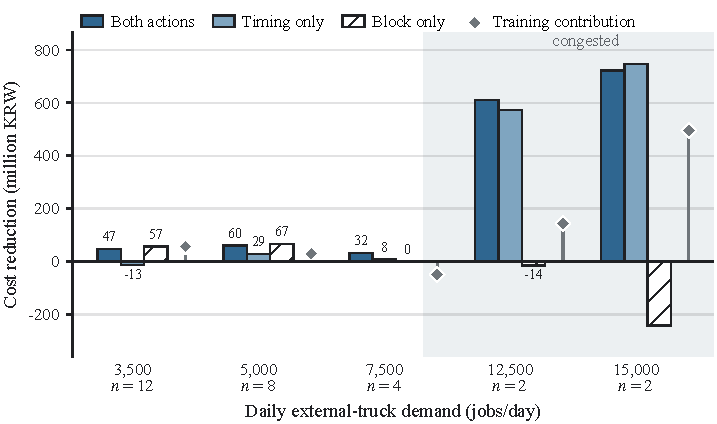
\includegraphics[width=\textwidth]{fig-decomposition.pdf}
\caption{Cost reduction by demand level, decomposed by action range, in
million KRW. The shaded band marks the two congested levels; because
those are more than ten times larger than the rest, the value is printed
next to each short bar, and $n$ is the number of days observed. Bars
measure a restricted policy against no reallocation, whereas the diamond
is the learned policy minus the first-iteration model and therefore
carries a different mark.}
\label{fig:decomp}
\end{figure}

\subsection{Effect of Learning and Sensitivity to the Dispatching Rule}
\label{sec:exp-learning}
Losses below are reported in the scaled label units of
Sect.~\ref{sec:arch-labels} as means over the first and last five of the 30
training iterations. The proposal network's Huber loss decreases from
0.079 to 0.029 on training decisions and from 0.268 to 0.119 on
validation decisions; the acceptance network decreases from 0.171 to
0.027 and from 0.315 to 0.136. The decline in
validation loss indicates that the learned mapping generalises to
held-out decisions, although the final validation loss remains about
four times the training loss; with about 56 labelled decisions per
iteration, this supports keeping the model small. The share of decisions
whose counterfactual difference is exactly zero falls from 51.4\% to
37.6\% as exploration decreases, and training used 4{,}671
counterfactual worlds in total (Fig.~\ref{fig:learn}).

\begin{figure}[bp]
\centering

\includegraphics[width=\textwidth]{fig-learning-curve-2p.pdf}
\caption{Training and validation loss over the 30 iterations, with the
per-iteration value drawn faintly beneath a five-iteration mean; the
vertical axis is logarithmic. Shading marks the iterations in which the
demand level drawn was 12{,}500 or above, so much of the visible
fluctuation follows that draw rather than the fit. Exploration decreased linearly
from 0.50 to 0.05.}
\label{fig:learn}
\end{figure}

The first-iteration model cost KRW 9.20\,billion over the same days, so the
remaining 29 iterations added KRW 0.675\,billion, or 45.9\% of the total
reduction. The trained model is cheaper on only 18 of 28 days
($p=0.185$), and the four congested days account for 94.6\% of this
increment, and the trained model is cheaper on all four. A stratified
bootstrap over the daily differences with 20{,}000 resamples gives a
95\% interval of $[-32,-17]$\,million per day for the mean difference, which
excludes zero: the learning effect is large in total and concentrated,
but not frequent enough for the day-level sign test at a conventional
significance level. Establishing it more firmly requires more congested
days rather than more days overall. Finally, the ranking of crane-dispatching rules changes with demand
---the shortest processing time rule is 22--25\% more expensive under
smooth demand but the cheapest from 7{,}500 trucks upward---so the
reallocation effect should also be tested under other rules.

% =====================================================================
\section{Conclusion}
\label{sec:concl}
This paper proposed a reinforcement learning architecture that revisits
the yard block and the arrival time of an already announced
external-truck job during operation. Independent proposal and acceptance
policies and a central commitment step connect distributed appointment
coordination~\cite{ref6} and yard-crane operation~\cite{ref7,ref8} into
one spatio-temporal assignment problem, and each policy learns from
counterfactual cost differences measured over a fixed horizon rather
than from an immediate movement cost; this brings multi-agent
counterfactual learning~\cite{ref10,ref11} into the operating decision.
Because the expensive branch simulation is used only during offline
training, online operation requires only small cost networks and
constraint checks. In the synthetic environment the architecture reduced
cost by 14.7\% against no reallocation and was cheaper than a rule with
the same action range on 20 of 28 days; the reduction came mainly from
arrival-time adjustment on congested days. Because a rule can be
cheaper on more days while the
learned policy is cheaper in total, both the frequency of lower-cost
outcomes and the aggregate reduction are needed for interpretation.
These results establish the architecture in a literature-based synthetic
environment rather than estimating performance at a particular terminal,
and the concentration of the effect on congested days suggests operating
the policy selectively rather than continuously. They rest on a
single 30-day realisation and carry no estimate of variation across
realisations. Future work will extend
the framework along three axes: terminal-specific arrival, demand, and
cost data; executable appointment quotas and alternative acceptance
structures, including the value of the acceptance veto; and robustness
across counterfactual horizons, cost structures, and crane-dispatching
rules.

% =====================================================================
\begin{credits}
\subsubsection{\ackname}
This work was supported by the Public-Private Joint Technology
Commercialization R\&D program (Technology Transfer and
Commercialization, RS-2026-25529952) funded by the Ministry of SMEs and
Startups (MSS, Korea).

\subsubsection{\discintname}
The authors have no competing interests to declare that are relevant to
the content of this article.
\end{credits}

% =====================================================================
\small
\begin{thebibliography}{18}
\setlength{\itemsep}{0pt}
\setlength{\parsep}{0pt}
\setlength{\topsep}{2pt}
\bibitem{ref1} Yen, B.T.H., Huang, M.J., Lai, H.J., Cho, H.H., Huang, Y.L.: How smart port design influences port efficiency: a DEA-Tobit approach. Res. Transp. Bus. Manag. \textbf{46}, 100862 (2023)
\bibitem{ref4} Chen, G., Govindan, K., Yang, Z.: Managing truck arrivals with time windows to alleviate gate congestion at container terminals. Int. J. Prod. Econ. \textbf{141}(1), 179--188 (2013)
\bibitem{ref6} Phan, M.-H., Kim, K.H.: Collaborative truck scheduling and appointments for trucking companies and container terminals. Transp. Res. B \textbf{86}, 37--50 (2016)
\bibitem{ref7} Ng, W.C., Mak, K.L.: Yard crane scheduling in port container terminals. Appl. Math. Model. \textbf{29}(3), 263--276 (2005)
\bibitem{ref8} Speer, U., Fischer, K.: Scheduling of different automated yard crane systems at container terminals. Transp. Sci. \textbf{51}(1), 305--324 (2017)
\bibitem{ref9} Petering, M.E.H., Murty, K.G.: Effect of block length and yard crane deployment systems on overall performance at a seaport container transshipment terminal. Comput. Oper. Res. \textbf{36}(5), 1711--1725 (2009)
\bibitem{ref16} Schwientek, A., Lange, A.-K., Jahn, C.: Simulation-based analysis of dispatching methods on seaport container terminals. In: ASIM Symp. Simulationstechnik (SST 2020). ARGESIM Report, vol.~59, pp. 357--364 (2020)
\bibitem{ref19} Wang, W., Liu, H., Peng, Y., Cao, Z., Yu, P., Lu, Z.: Yard crane real-time scheduling among multi-block at terminal: A reinforcement learning based proximal policy optimization approach. Transp. Res. E \textbf{207}, 104635 (2026)
\bibitem{ref10} Wolpert, D.H., Tumer, K.: Optimal payoff functions for members of collectives. Adv. Complex Syst. \textbf{4}(2--3), 265--279 (2001)
\bibitem{ref11} Foerster, J.N., Farquhar, G., Afouras, T., Nardelli, N., Whiteson, S.: Counterfactual multi-agent policy gradients. In: Proc. 32nd AAAI Conf. Artif. Intell. pp. 2974--2982. AAAI Press (2018)
\bibitem{ref13} Kourounioti, I., Polydoropoulou, A.: Application of aggregate container terminal data for the development of time-of-day models predicting truck arrivals. Eur. J. Transp. Infrastruct. Res. \textbf{18}(1), 76--90 (2018)
\bibitem{refmnih} Mnih, V., et al.: Human-level control through deep reinforcement learning. Nature \textbf{518}(7540), 529--533 (2015)
\bibitem{refhornik} Hornik, K.: Approximation capabilities of multilayer feedforward networks. Neural Netw. \textbf{4}(2), 251--257 (1991)
\bibitem{refhuber} Huber, P.J.: Robust estimation of a location parameter. Ann. Math. Statist. \textbf{35}(1), 73--101 (1964)
\bibitem{ref20} Kim, S., Mowakeaa, R., Kim, S.-J., Lim, H.: Building energy management for demand response using kernel lifelong learning. IEEE Access \textbf{8}, 82131--82141 (2020)
\bibitem{ref25} Ministry of Oceans and Fisheries: Regulations on the Use of Port Facilities and Fees at Trade Ports, etc. MOF Notice No. 2025-218 (2025) (in Korean)
\bibitem{ref24} Ministry of Land, Infrastructure and Transport: Notice on Safe Freight Rates for Cargo Vehicles Applicable in 2026. MOLIT Notice No. 2026-402 (2026) (in Korean)
\bibitem{ref22} Kleijnen, J.P.C.: Analyzing simulation experiments with common random numbers. Manag. Sci. \textbf{34}(1), 65--74 (1988)
\end{thebibliography}

\end{document}
